% ======================================================================
%  latexmk -xelatex lab2.tex
% ======================================================================
\documentclass[a4paper,12pt]{article}
\usepackage{mai-report}

\usepackage{graphicx}

% ======================================================================
\renewcommand{\reportNumber}{2}
\renewcommand{\reportDiscipline}{Операционные системы и архитектура компьютера}
\renewcommand{\reportTheme}{\textit{[Название темы лабораторной работы]}}
\renewcommand{\reportStudent}{Черноглазкин Е.А.}
\renewcommand{\reportGroup}{206}
\renewcommand{\reportTeacher}{Ефимов Д.А.}
\renewcommand{\reportTeacherRole}{Ассистент Центра ТОП-ИТ}
\renewcommand{\reportCity}{Москва}
\renewcommand{\reportYear}{2026}

\begin{document}

\maketitlepage

% ======================================================================
\section{Цель работы}

\textit{Приобретение практических навыков в управление процессами в ОС и обеспечение обмена данных между процессами посредством каналов.}

% ======================================================================
\section{Краткое описание архитектуры решения}

\textit{Реализована программа, состоящая из трёх процессов: основного (родительского) и двух дочерних. Программа выполняет чтение строки произвольной длинны, введённой пользователем, после чего выполняет замену всех заглавных букв в переданной строке на маленькие и убирает парные пробелы. За чтение и вывод результата отвечает родительский процесс. За понижение регистра символов - первый ребёнок, за схлопывание пробелов - второй ребёнок.}

\subsection{Схема взаимодействия компонентов}

\begin{center}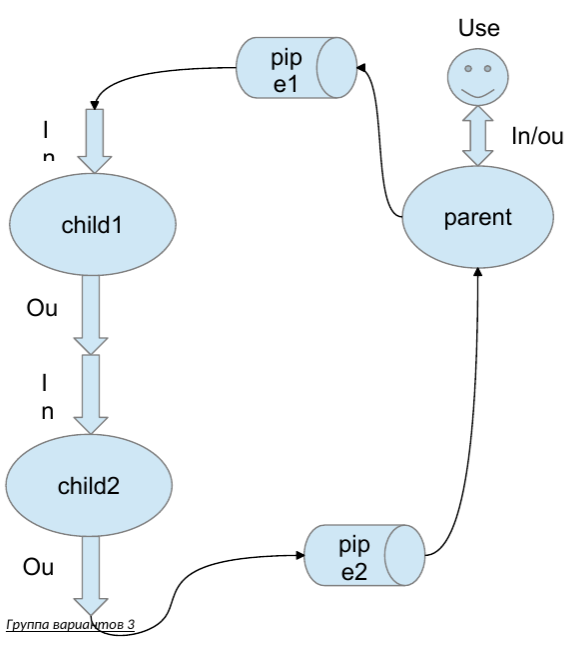
\includegraphics[width=0.8\linewidth]{scheme.png}\end{center}

\figcaption{Архитектура решения}

% ======================================================================
\section{Листинг ключевых фрагментов кода}

\textit{Далее рассматриваются основные фрагменты кода, разделённые на 4 файла.}

\subsection{Функция записи в пайп}

\textit{Функция реализует запись в пайп и вынесена в отдельный файл, так как используется во всех 3-х программах процессов. Функция выполняет запись в пайп по указанному дескриптору, обрабатывает завершение записи в случае возникновения ошибки, кроме случаев, когда ошибка вызвана прерыванием системного вызова сигналом. В случае прерывания функция возобновляет свою работу и продолжает запись с того места, где остановилась.}

\begin{codeblock}
...
int write_to_pipe(int pipe_fd, char *mem, size_t write_index) {
    ssize_t bytes_written = 0, bytes_written_total = 0;
    while (write_index - bytes_written_total > 0) {
        bytes_written = write(pipe_fd, mem + bytes_written_total, write_index - bytes_written_total);

        if (bytes_written == -1) {
            if (errno == EINTR) {
                continue;
            }
            return 1;
        }

        bytes_written_total += bytes_written;
    }
    return 0;
}
...
\end{codeblock}
\lstcaption{Запись в пайп}


\subsection{wait_for_child_status}

\textit{Функция реализует ожидания ответа от завершения дочернего процесса и обработку его статуса. Если процесс завершился сам (WIFEXITED), то WEXITSTATUS получает его код и делает вывод в зависимости от его значения. Если ребёнок был убит сигналом (WIFSIGNALED), выводится код сигнала при помоши WTERMSIG.}

\begin{codeblock}
...
int wait_for_child_status(pid_t pid, const char *child_name) {
    int status;
    if (waitpid(pid, &status, 0) == -1) {
        perror("Waitpid failed");
        return 1;
    }

    if (WIFEXITED(status)) {
        int exit_code = WEXITSTATUS(status);

        if (exit_code == ERR_EXEC_FAILED) {
            fprintf(stderr, "Child (%s) was unable to execute exec.\n", child_name);
            return 1;
        } else if (exit_code == ERR_SETUP_FAILED) {
            fprintf(stderr, "Child (%s) failed to set up file descriptors and never started.\n", child_name);
            return 1;
        } else if (exit_code != 0) {
            fprintf(stderr, "Child (%s) started but finished with an error.\n", child_name);
            return 1;
        }
    } else if (WIFSIGNALED(status)) {
        fprintf(stderr, "Child (%s) process was killed with a signal %d.\n", child_name, WTERMSIG(status));
        return 1;
    }
    return 0;
}
...
\end{codeblock}
\lstcaption{Обработка завершения дочернего процесса}


\subsection{print_from_pipe}

\textit{Функция отвечает за вывод результата, который второй дочерний процесс отправил в pipe между ним и родителем. Происходит чтение или ожидание поступления информации в пайп до тех пор, пока не будет возвращён 0, сообщающий о том, что писателей больше не осталось (второй ребёнок завершился). В случае ошибки (-1) обрабатывает её и выходит, кроме случая, когда происходит прерывание системного вывода пришедшим сигналом - в таком случае работа функции продолжается.}

\begin{codeblock}
...
int result = 0;
ssize_t bytes_read;
while ((bytes_read = read(pipe_fd, buffer, block_size)) != 0) {
    if (bytes_read == -1) {
        if (errno == EINTR) {
            continue;
        }
        perror("Read from pipe failed");
        result = 1;
        break;
    }
    fwrite(buffer, 1, bytes_read, stdout);
}
...
\end{codeblock}
\lstcaption{Вывод результата работы}


\subsection{Настройка пайпов}

\textit{В соответствии с описанной ранее схеме, в начале своей работы родительский процесс подготавливает дескрипторы и создаёт пайпы. В случае возникновения ошибки она обрабатывается и происходит завершение процесса через exit.}

\begin{codeblock}
...
int par_to_ch_pipe_fd[2], ch_to_ch_pipe_fd[2], ch_to_par_pipe_fd[2];
if (pipe(par_to_ch_pipe_fd) == -1) {
    perror("Pipe");
    exit(EXIT_FAILURE);
}
if (pipe(ch_to_ch_pipe_fd) == -1) {
    perror("Pipe");
    exit(EXIT_FAILURE);
}
if (pipe(ch_to_par_pipe_fd) == -1) {
    perror("Pipe");
    exit(EXIT_FAILURE);
}
...
\end{codeblock}
\lstcaption{Создание пайпов}


\subsection{Запуск дочернего процесса}

\textit{Запуск дочерних процессов аналогичен и отличается только подключениями и значениями execv. Выполняется форк для создания копии родителя, в случае ошибки она обрабатывается. Для форкнутого процесса (он продолжает работу с того же места), получающего pid 0 выполняется подготовка окружения: перенастройка нужных и закрытие ненужных дескрипторов, которые были у родителя так, чтобы далее запускаемая через execv дочерняя программа могла работать не зная о своём родителе (stdin = чтение из пайпа, stdout = запись в другой пайп). Для запуска процесса используется execv, который передаёт параметры окружения автоматически, а остальное задаётся в коде (название и путь к бинарному файлу).}

\begin{codeblock}
...
pid1 = fork();
if (pid1 == -1) {
    perror("Fork 1");
    exit(EXIT_FAILURE);
}
else if (pid1 == 0) {
    // Child1 process
    if (dup2(par_to_ch_pipe_fd[0], 0) == -1) {
        perror("Dup2");
        _exit(ERR_SETUP_FAILED);
    }
    if (dup2(ch_to_ch_pipe_fd[1], 1) == -1) {
        perror("Dup2");
        _exit(ERR_SETUP_FAILED);
    }

    close(par_to_ch_pipe_fd[0]); close(par_to_ch_pipe_fd[1]);
    close(ch_to_ch_pipe_fd[0]); close(ch_to_ch_pipe_fd[1]);
    close(ch_to_par_pipe_fd[0]); close(ch_to_par_pipe_fd[1]);

    char *lower_name = "lower";
    char *lower_path = "./lower";
    char *args[] = {lower_name, NULL};
    execv(lower_path, args);

    perror("Execv failed");
    _exit(ERR_EXEC_FAILED);
}
...
\end{codeblock}
\lstcaption{Запуск дочернего процесса}


\subsection{Описание реакции на сигнал}

\textit{Создаётся структура для указания параметров реакции процесса на приходящие ему сигналы. В случае родителя структура обнуляется во избежании попадания туда мусора. Выставляется SIG_IGN - режим игнорирования и маска блокировки сигналов (которая, правда, при режиме игнорирования не то чтобы имеет значение, но аккуратность не будет лишней). После этого устанавливается реакция на SIGPIPE - ошибка записи в пайп из-за отсутствия у него хотя бы одного читателя. В таком случае мы продолжаем работу программы, чтобы получить статусы детей и узнать, что произошло с первым ребёнком, из-за чего он перестал читать.}

\begin{codeblock}
...
struct sigaction sa = {0};
sa.sa_handler = SIG_IGN;
sigemptyset(&sa.sa_mask);
if (sigaction(SIGPIPE, &sa, NULL) == -1) {
    perror("sigaction");
}
...
\end{codeblock}
\lstcaption{Реакция на сигнал}


\subsection{Чтение и запись}

\textit{Основной логикой родителя является чтение пользовательского ввода, запись его в пайп и вывод результата работы детей из пайпа обратно пользователю. За это отвечают ранее рассмотренные функции, а также их обёртки, обрабатывающие ошибки их работы. Попутно с этим выполняются обычные обработки ошибок (выделение памяти, ошибки записи, чтения, обработка статусов детей и так далее). Подробнее с этим можно ознакомиться в полном коде программы.}

\begin{codeblock}
...
size_t input_length = 0;
char *input_string = dynamic_input_reading(stdin, &input_length);
if (!input_string) {
    fprintf(stderr, "Memory allocation for input failed.\n");
    result |= ERR_FLAG_MEM;
}

if (input_string) {
    if (write_to_pipe(par_to_ch_pipe_fd[1], input_string, input_length) != 0) {
        if (errno == EPIPE) {
            fprintf(stderr, "Child 1 (lower) stopped accepting input.\n");
        } else {
            perror("Write to child 1 failed");
        }
        result |= ERR_FLAG_WRITE;
    }
}
close(par_to_ch_pipe_fd[1]);

size_t block_size = 1024;
if (print_from_pipe(ch_to_par_pipe_fd[0], block_size)) {
    result |= ERR_FLAG_IO;
}
close(ch_to_par_pipe_fd[0]);
...
\end{codeblock}
\lstcaption{Чтение и запись строк}

\subsection{Дети}

\textit{Код детей можно прочитать в полном коде, в рамках отчёта на основании всего вышеописанного приму его как тривиальный. Дети читают, пока читается, обрабатывают и пишут, пока пишется, попутно проверяя корректность выполняемых операций.}

% ======================================================================
\section{Результаты работы}

\subsection{Консольный вывод или логи}

\begin{codeblock}
root@inchanterx:~/os_labs_sem3/lab2# ./parent
Input desired string: HELLO! I really  really    want this program to work, therefore I could go to make myself a breakfast...
hello! i really really want this program to work, therefore i could go to make myself a breakfast...
\end{codeblock}

\textit{Введённая строка корректно обрабатывается и выводится в соответствии с требованиями.}

\subsection{Скриншоты результатов}

\begin{center}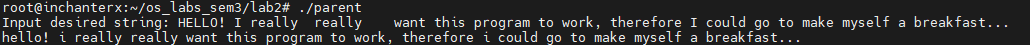
\includegraphics[width=0.8\linewidth]{result.png}\end{center}

\figcaption{Подтверждение работоспособности программы}

% ======================================================================
\section{Выводы}

\textit{[В результате проделанной работы была написана программа, использующая системные вызовы для создания дочерних процессов для выполнения понижения регистра символов в тексте и устранения излишних пробелов. Были получены практические навыки создания процессов, пайпов и обработки сигналов и ошибок.]}

\end{document}
